\chapter{Estado del Arte}

\section{Diseño e Implementación de SR}
Los modelos de difusión \autocite{NEURIPS2020_4c5bcfec} han superado recientemente a los modelos GAN \autocite{NIPS2014_5ca3e9b1} en el estado del arte de metodologías generativas de imágenes \autocite{10081412}. Aunque los GAN han sido utilizados ampliamente en superresolución de imágenes \autocite{9044873}, su proceso de entrenamiento es delicado y tiende a ser inestable. En contraste, los modelos de difusión, que también son probabilísticos y generan resultados a partir de una distribución de probabilidad, han demostrado ser más fáciles de entrenar y producir mejores resultados, superando a otras metodologías en muchas métricas de reconstrucción \autocite{saharia2021image}. Este desarrollo también ha sido reconocido en la comunidad de teledetección, con artículos recientes sobre superresolución que han adoptado metodologías de SR basadas en difusión \autocite{rs14194834, 10057005, 103389fmars20231211981}.

\begin{figure}[H]
    \caption{\doublespacing \\ \textit{Modelos de difusión en el espacio de píxeles (arriba) y en el espacio latente (abajo).}} 
    \centering
    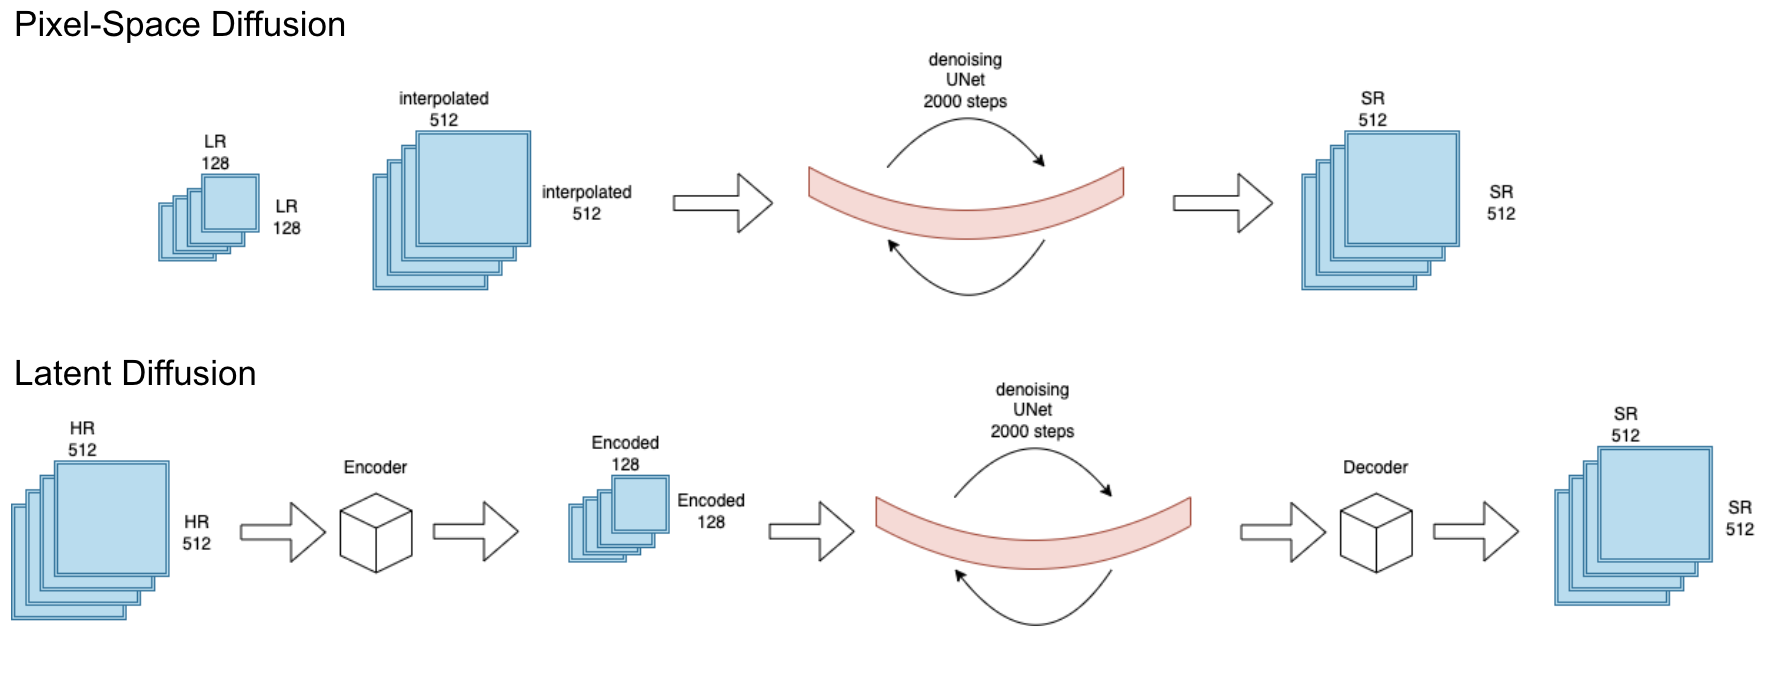
\includegraphics[width=1\linewidth]{images/lat_px_dif.png}
    \begin{justify}
        \textit{Nota.} Modelos de difusión en el espacio de píxeles (arriba) y en el espacio latente (abajo).
    \end{justify}                    
    \label{fig:pixel_latent_space}
\end{figure}

\subsection{Difusión en Espacio Latente vs Difusión en Espacio de Píxeles}

La mayoría de los modelos de SR en la literatura emplean difusión en el espacio de píxeles (ver Figura \ref{fig:pixel_latent_space}, arriba). En este flujo de trabajo, la imagen $LR$ se interpola al tamaño deseado y se somete a un U-Net de eliminación de ruido, que pasa \textit{n} veces, eliminando una pequeña cantidad de ruido en cada iteración. Este método es computacionalmente costoso, ya que cada imagen que necesita ser superresuelta debe pasar muchas veces por toda la red para obtener el resultado. Generalmente, se utilizan entre 500 y 2000 iteraciones.

Los modelos de difusión en espacio latente, en cambio, realizan los pasos de eliminación de ruido en una representación de menor dimensión de la imagen de entrada (ver Figura \ref{fig:pixel_latent_space}, abajo). Una red separada, el autoencoder, genera un espacio latente más pequeño que el espacio de entrada original, haciendo que el paso de eliminación de ruido sea mucho más rápido. Después de la eliminación de ruido, la imagen es decodificada y expandida nuevamente a la dimensionalidad original deseada del producto SR. Se ha demostrado que realizar difusión en el espacio latente reduce significativamente los requisitos computacionales al tiempo que preserva las potentes capacidades de SR de los modelos de difusión \autocite{rombach2022highresolution}.

\subsection{Código Base}

Se han desarrollado varias bases de código relacionadas con modelos de superresolución (SR) disponibles para exploración e implementación (ver Figura \ref{fig:codebase}). Entre ellas, destacan dos implementaciones no oficiales del modelo SR3 \autocite{saharia2021image}, una en \href{https://github.com/Janspiry/Image-Super-Resolution-via-Iterative-Refinement}{GitHub de Janspiry} y otra de \href{https://github.com/KiUngSong/Generative-Models/tree/main/SR3}{KiUngSong}. Estas repositorios brindan valiosa información sobre la funcionalidad de SR3, aunque se centran en la difusión en el espacio de píxeles y han recibido comentarios de la comunidad sobre ciertas decisiones de diseño y limitaciones en la calidad del código y su capacidad de expansión. Además, estas implementaciones tienden a producir resultados de calidad media.

\begin{figure}[H]
    \caption{\doublespacing \\ \textit{Bases de código en uso.}} 
    \centering
    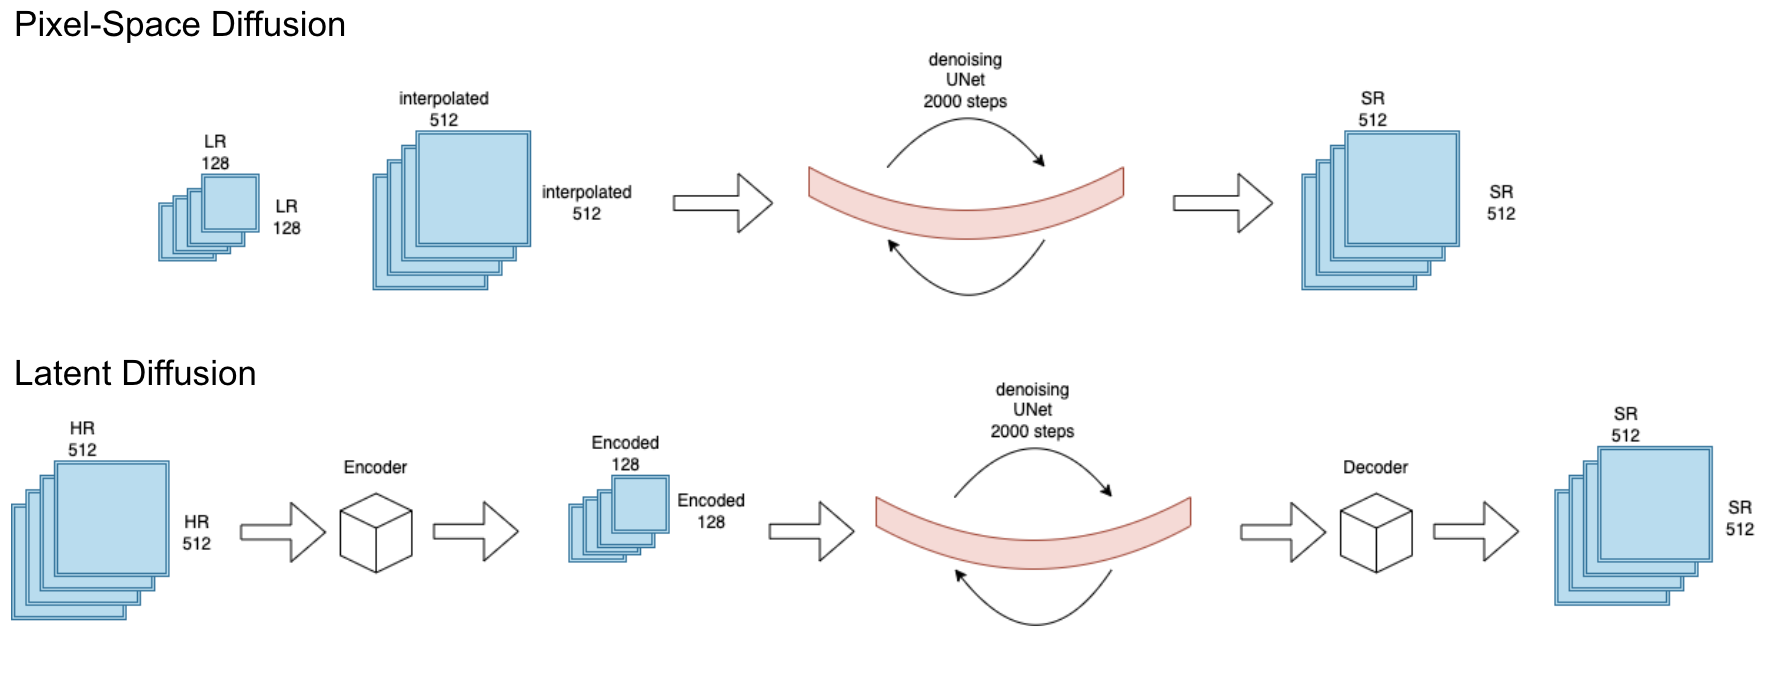
\includegraphics[width=1\linewidth]{images/lat_px_dif.png}
    \begin{justify}
        \textit{Nota.} Bases de código en uso.
    \end{justify}                    
    \label{fig:codebase}
\end{figure}

Otro recurso destacado es el repositorio \href{https://github.com/mikonvergence/DiffusionFastForward}{DiffusionFastForward}, que sirve como una implementación tipo tutorial clara para modelos de difusión tanto en el espacio de píxeles como en el espacio latente. Sin embargo, es relativamente simple y depende en gran medida de repositorios externos, lo que limita su escalabilidad y modificabilidad. A pesar de su simplicidad, ofrece una buena comprensión de las estrategias básicas de difusión para SR.

Finalmente, el repositorio de \href{https://github.com/mikonvergence/DiffusionFastForward}{latent-diffusion}, el código oficial del exitoso modelo de difusión en el espacio latente \autocite{rombach2022highresolution}, ofrece una solución integral que abarca diversas tareas como la generación incondicional de imágenes, la generación de imágenes basadas en texto, inpainting y superresolución. Este repositorio es conocido por su versatilidad y estructura bien organizada, lo que lo hace altamente adaptable para modificaciones y expansiones. La disponibilidad de puntos de control preentrenados proporcionados por los autores también permite una demostración inmediata de las sólidas capacidades del modelo, posicionándolo como un recurso líder para proyectos de superresolución.


\subsection{Autoencoder}

El autoencoder en consideración está diseñado para comprimir la dimensión espacial por un factor de 4, reduciendo tensores de \textit{4$\times$512$\times$512} a \textit{4$\times$128$\times$128} antes de decodificarlos de nuevo a sus dimensiones originales. Este enfoque está inspirado en el repositorio de \textit{latent-diffusion}, como se describe en \autocite{rombach2022highresolution}. Idealmente, tales procesos de codificación y decodificación buscan preservar la calidad de la imagen. Más allá de las métricas de reconstrucción, el espacio latente producido por el autoencoder desempeña un papel crucial en la superresolución, ya que la eliminación de ruido ocurre después del codificador. Este tipo de autoencoder ha sido utilizado con éxito en varias aplicaciones, como lo demuestra el modelo de difusión latente y sus adaptaciones en investigaciones anteriores \autocite{esser2021taming}.

En este contexto, los modelos suelen entrenarse independientemente del U-Net de eliminación de ruido, utilizando una combinación de LPIPS perceptual y un componente GAN. El componente GAN generalmente emplea un clasificador que distingue entre imágenes reales e imágenes reconstruidas, donde los logits de salida se combinan con la pérdida perceptual y luego se retropropagan a través del autoencoder. La métrica LPIPS \autocite{zhang2018unreasonable} es ampliamente utilizada en tareas de visión por computadora, simulando la percepción visual humana para devolver un puntaje de similitud entre dos imágenes. Dado que LPIPS se basa en una red VGG \autocite{simonyan2015deep} y está entrenada principalmente en datos RGB, extenderla para manejar más de 3 bandas presenta desafíos, especialmente para modelos de 4 bandas como RGB-NIR. En tales casos, una solución común implica seleccionar 3 bandas al azar en cada paso de entrenamiento y alimentarlas al modelo LPIPS. Aunque poco convencional, este método ha sido validado, ya que las permutaciones aleatorias del tensor de 4 bandas en 3 bandas no han mostrado una pérdida significativa en la precisión de LPIPS. La Figura \ref{fig:lpips_permutation} demuestra que los resultados en boxplots de LPIPS para 200 pares de imágenes LR-HR interpoladas permanecen consistentes, incluso cuando se utilizan combinaciones de bandas espectrales que no formaban parte del entrenamiento original, lo que respalda la viabilidad de este enfoque.

\begin{figure}[H]
    \caption{\doublespacing \\ \textit{Boxplots de LPIPS para todas las permutaciones posibles de 3 bandas a partir de tensores de 4 bandas.}} 
    \centering
    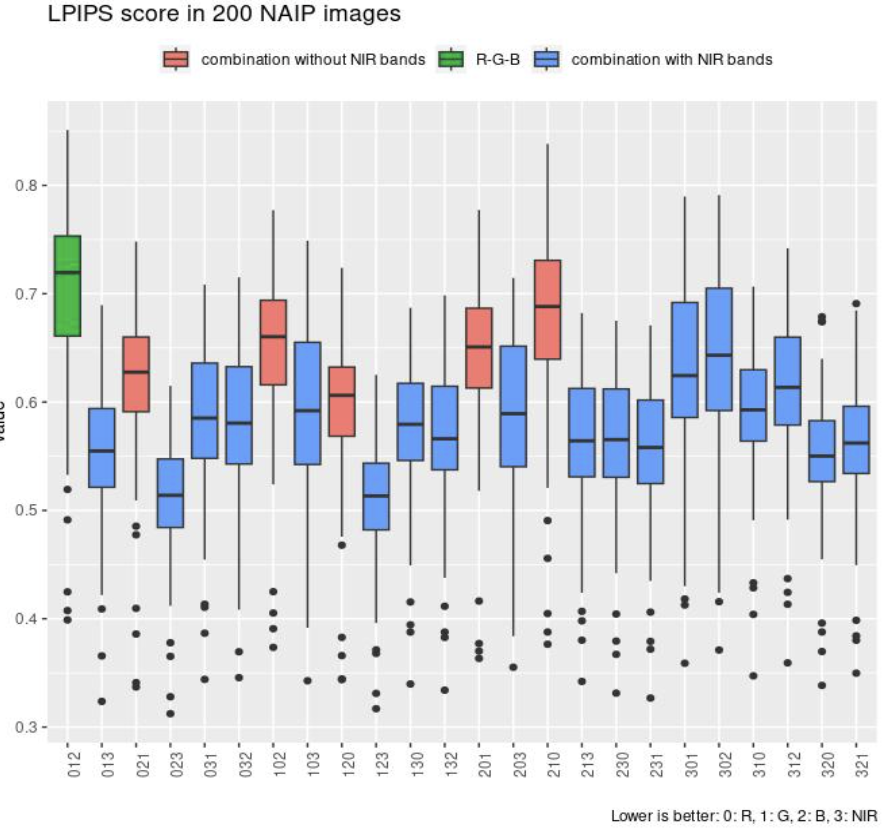
\includegraphics[width=1\linewidth]{images/lpips_permutation.png}
    \begin{justify}
        \textit{Nota.} Boxplots de LPIPS para todas las permutaciones posibles de 3 bandas a partir de tensores de 4 bandas.
    \end{justify}                    
    \label{fig:lpips_permutation}
\end{figure}

\begin{figure}[H]
    \caption{\doublespacing \\ \textit{Valor mínimo (rojo claro), promedio (naranja), desviación estándar (verde) y máximo (azul) de los rangos de valores codificados.}} 
    \centering
    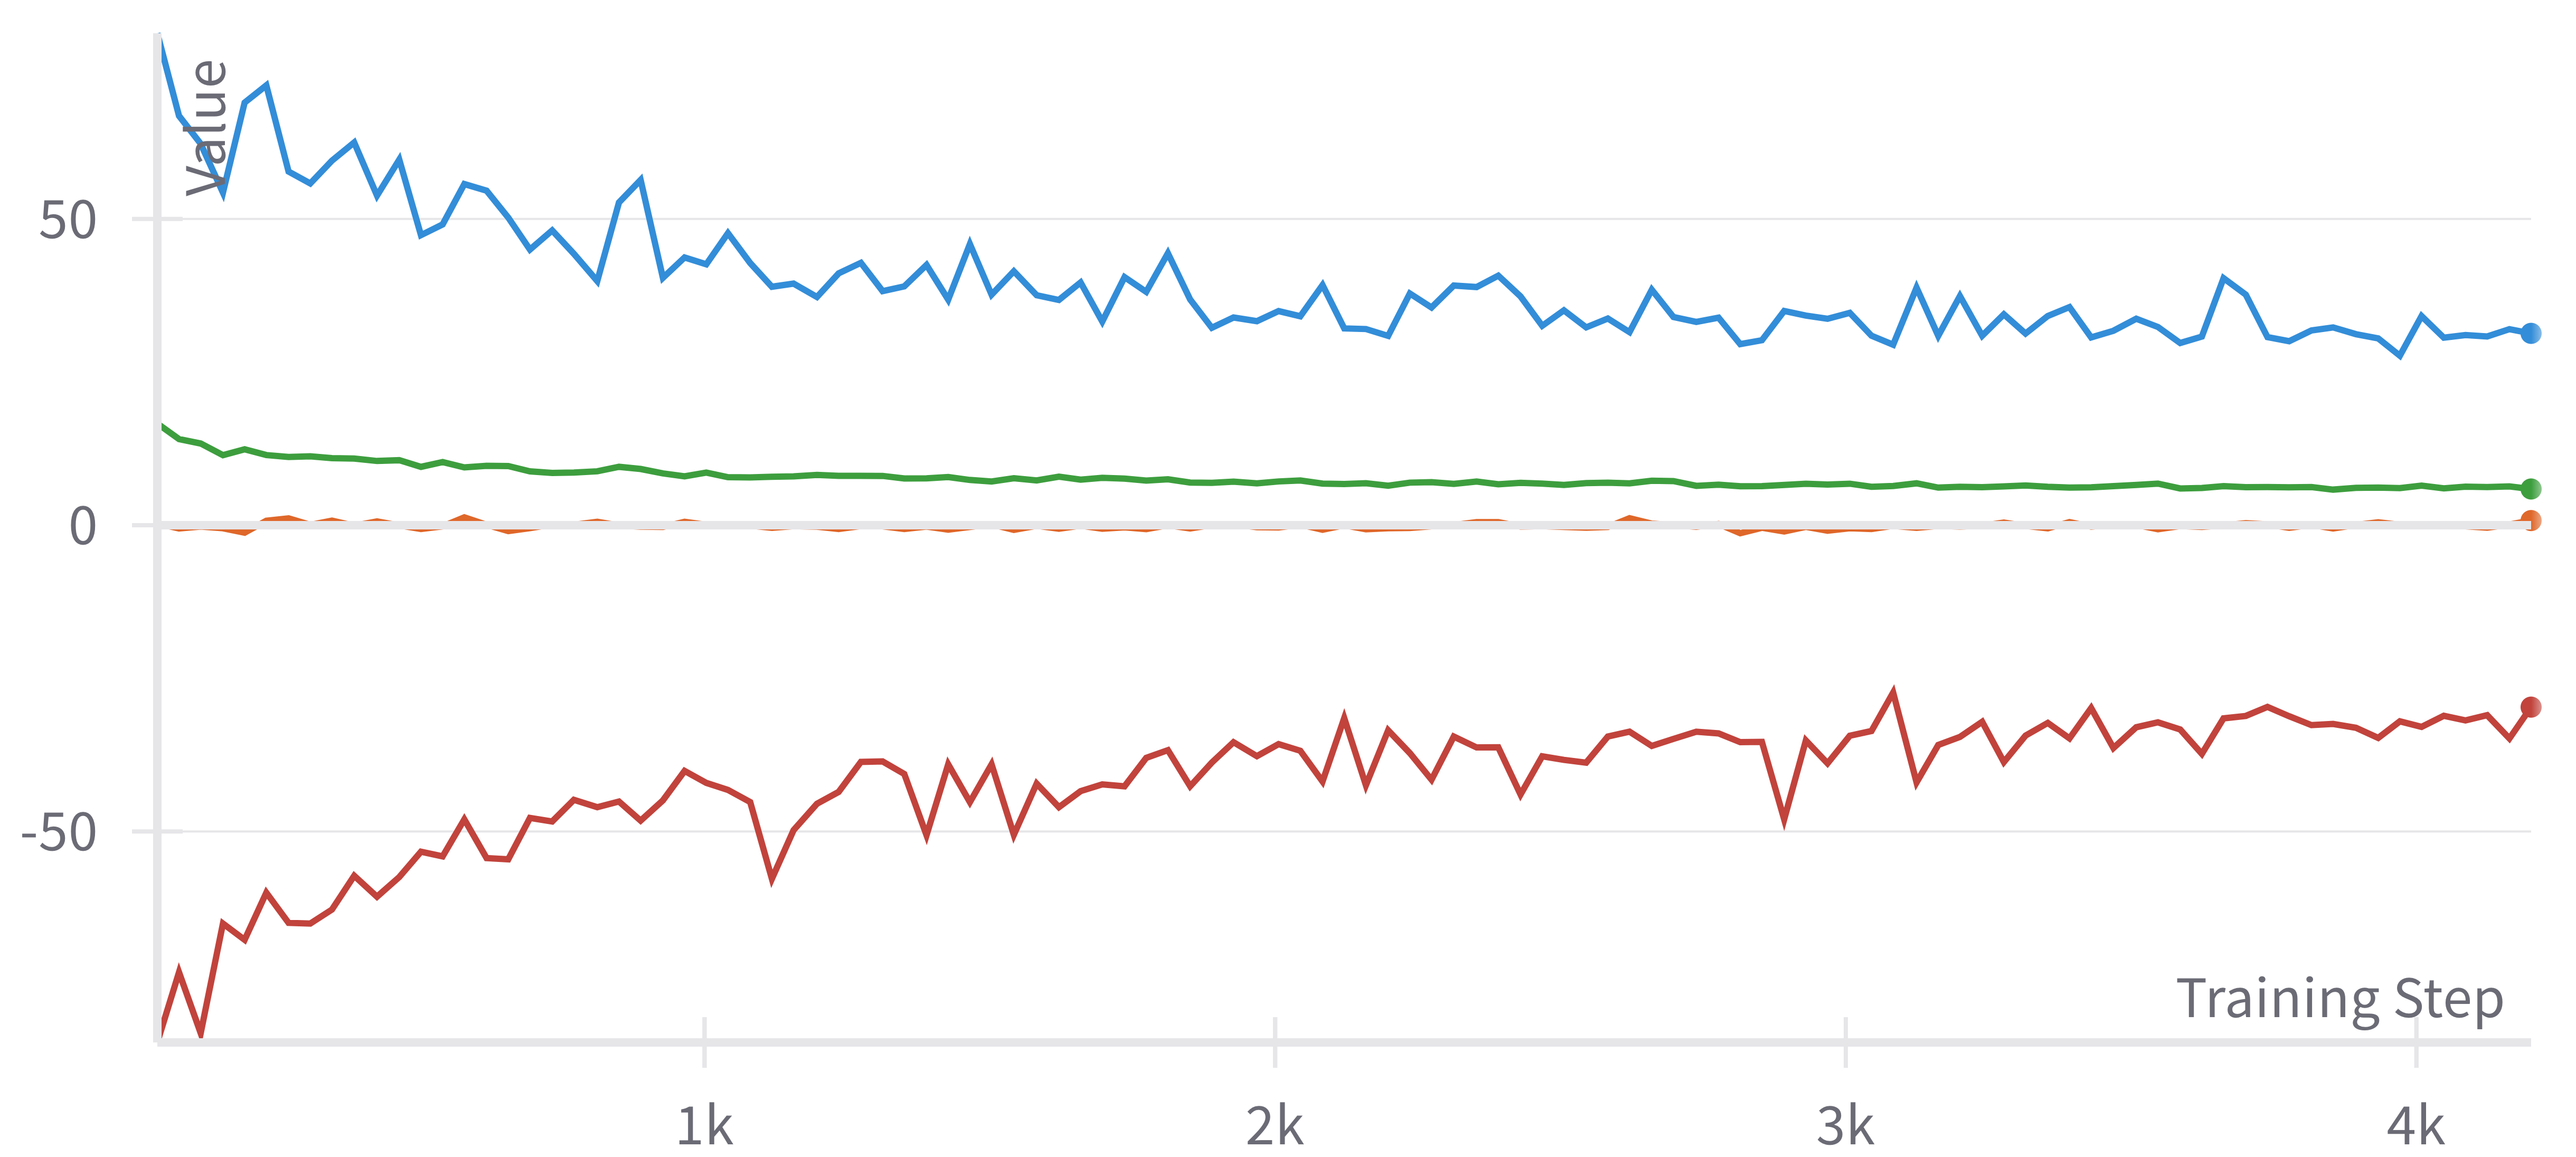
\includegraphics[width=1\linewidth]{images/simon/ae_distr_enc.png}
    \begin{justify}
        \textit{Nota.} Valor mínimo (rojo claro), promedio (naranja), desviación estándar (verde) y máximo (azul) de los rangos de valores codificados durante el entrenamiento del AE. La compresión excesiva del rango de valores afecta la precisión de la reconstrucción.
    \end{justify}                    
    \label{fig:ae_distr_enc}
\end{figure}

Además, se utiliza un autoencoder con regularización de Kullback-Leibler para asegurar que el espacio latente se asemeje al de la imagen de entrada. Esta regularización penaliza al codificador cuando la imagen codificada se desvía significativamente de la distribución original, lo cual es esencial durante la inferencia, donde el proceso de codificación se omite y la imagen se super-resuelve directamente desde dimensiones $LR$ de \textit{128$\times$128} a $HR$ de \textit{512$\times$512}. Mantener la distribución de valores codificados cercana a la de la imagen $LR$ (menos el ruido) es clave para lograr resultados de alta calidad.

Equilibrar la regularización de los valores codificados es fundamental para asegurar que la imagen codificada se mantenga similar a la de entrada, mientras se captura suficiente variación. La sobre-regularización, como reducir excesivamente los extremos o la desviación estándar del espacio latente, puede degradar la calidad de la reconstrucción (ver Figura \ref{fig:ae_distr_enc}). La evidencia empírica sugiere que una desviación estándar cercana a 5 logra un balance óptimo. Al utilizar números de punto flotante de 32 bits, este proceso traduce efectivamente parte de la complejidad espacial de alta resolución en representación numérica. Sin esta complejidad, la calidad de la reconstrucción se ve afectada.

Entrenar el autoencoder (AE) es un proceso delicado. Aunque la salida del decodificador converge rápidamente —reconstruyendo visualmente la imagen de entrada—, el modelo resultante no está listo de inmediato para integrarse en el flujo de trabajo de superresolución (SR). El componente GAN requiere un período de calentamiento antes de que su pérdida sea ponderada, y la regularización necesita tiempo para hacer efecto. Además, el autoencoder necesita una gran cantidad de datos de imágenes satelitales debido a su tamaño, con más de 72 millones de parámetros.

\begin{figure}[H]
    \caption{\doublespacing \\ \textit{Visualización de la imagen original, la imagen codificada y la imagen recuperada (de izquierda a derecha).}} 
    \centering
    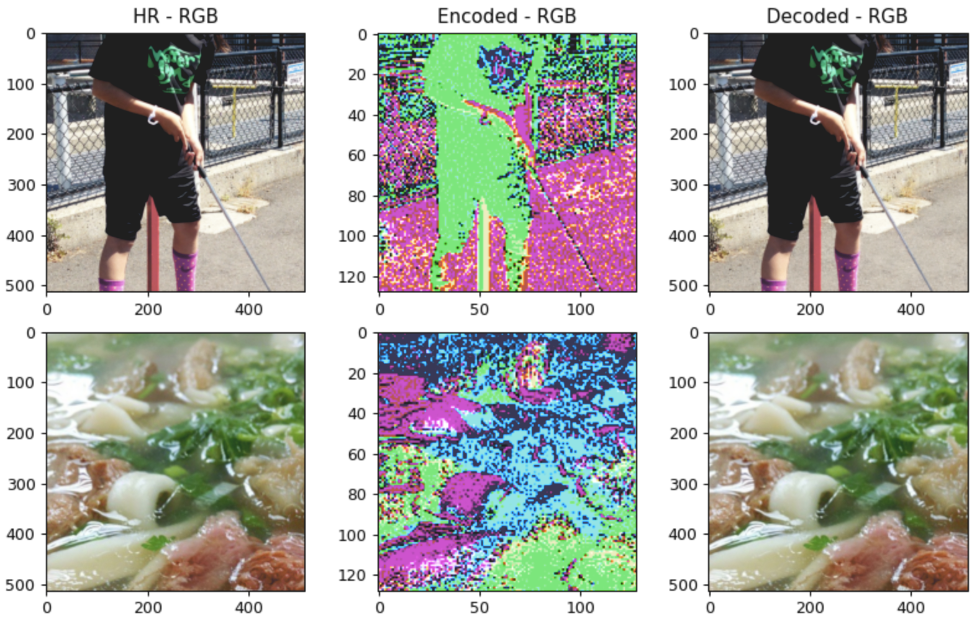
\includegraphics[width=1\linewidth]{images/autoencoder.png}
    \begin{justify}
        \textit{Nota.} Visualización de la imagen original, la imagen codificada y la imagen recuperada (de izquierda a derecha).
    \end{justify}                    
    \label{fig:autoencoder}
\end{figure}

La Figura \ref{fig:autoencoder} ilustra que, si bien la imagen se reconstruye fielmente, el espacio latente podría no estar optimizado para SR con el U-Net. Es necesario un entrenamiento exhaustivo, esquemas de tasa de aprendizaje cuidadosos y períodos de calentamiento, junto con la regularización del espacio latente, para evitar este problema.

\subsection{UNet de Eliminación de Ruido}
El modelo probabilístico de eliminación de ruido está diseñado para predecir iterativamente una versión sin ruido de la imagen de entrada aprendiendo la distribución de los datos de entrada. Este proceso puede describirse como una cadena de Markov, donde cada paso determina tanto el estado precedente como el siguiente. Al aprender la distribución $p(x)$ de los datos de entrada, el modelo puede revertir la cadena y producir imágenes sin ruido. El entrenamiento minimiza la cota inferior variacional en el logaritmo de la probabilidad de los datos bajo el modelo, penalizando las salidas que se encuentran en el extremo inferior de la escala de probabilidad respecto a la distribución objetivo.

El modelo de eliminación de ruido usa una arquitectura U-Net, aumentada con funciones de adición de ruido que manejan tanto la adición como la eliminación de ruido distribuido normalmente. Dado que el autoencoder realiza una escalación 4x, el modelo puede condicionarse a la imagen $LR$. En lugar de partir de una imagen de ruido puro, el proceso de eliminación de ruido comienza con la imagen $LR$ y va eliminando progresivamente el ruido, recuperando calidad antes de que la imagen sea escalada por el autoencoder. Este enfoque ha sido demostrado con éxito por \autocite{rombach2022highresolution} en varias tareas, como la generación incondicional de imágenes, el inpainting, la transferencia de estilo y la superresolución. En este flujo de trabajo, el U-Net se condiciona en la imagen $LR$ en el dominio espectral original, específicamente en el espacio de color RGB-NIR (ver Figura \ref{fig:encLR_schema}).

\subsubsection{Adaptaciones del UNet}
Dado que el proceso de muestreo del autoencoder espera una distribución similar a la de su propio entrenamiento (ver Figura \ref{fig:ae_distr_enc}), el U-Net aprende implícitamente a transformar la distribución espectral de entrada en la distribución espectral codificada. Aunque esta transformación no afecta la reconstrucción de características espaciales, sí impacta en la consistencia espectral de la imagen SR. Para mitigar esto, interpolamos la imagen $LR$ a las mismas dimensiones que la imagen $HR$ antes de codificarla. Este cambio libera al U-Net de la carga de aprender la correspondencia entre los dos dominios espectrales (Figura \ref{fig:encLR_schema}). Durante el entrenamiento, esto resulta en un condicionamiento que concatena el tensor $HR$ codificado con ruido con la imagen $LR$ de mismo tamaño, en lugar de mezclar dominios espectrales. En la inferencia, la imagen $HR$ codificada se reemplaza solo con el tensor de ruido del scheduler.

La experimentación demuestra que la imagen $LR$ interpolada puede codificarse y decodificarse fácilmente mediante el autoencoder, a pesar de que el AE se entrenó en imágenes $HR$ (Figura \ref{fig:encLRint_demo}). Aunque esto agrega un paso adicional a través del AE, no incrementa significativamente el tiempo de procesamiento durante el entrenamiento o la inferencia.

\begin{figure}[H]
    \caption{\doublespacing \\ \textit{Esquema de los cambios en el flujo de trabajo de SR del UNet.}} 
    \centering
    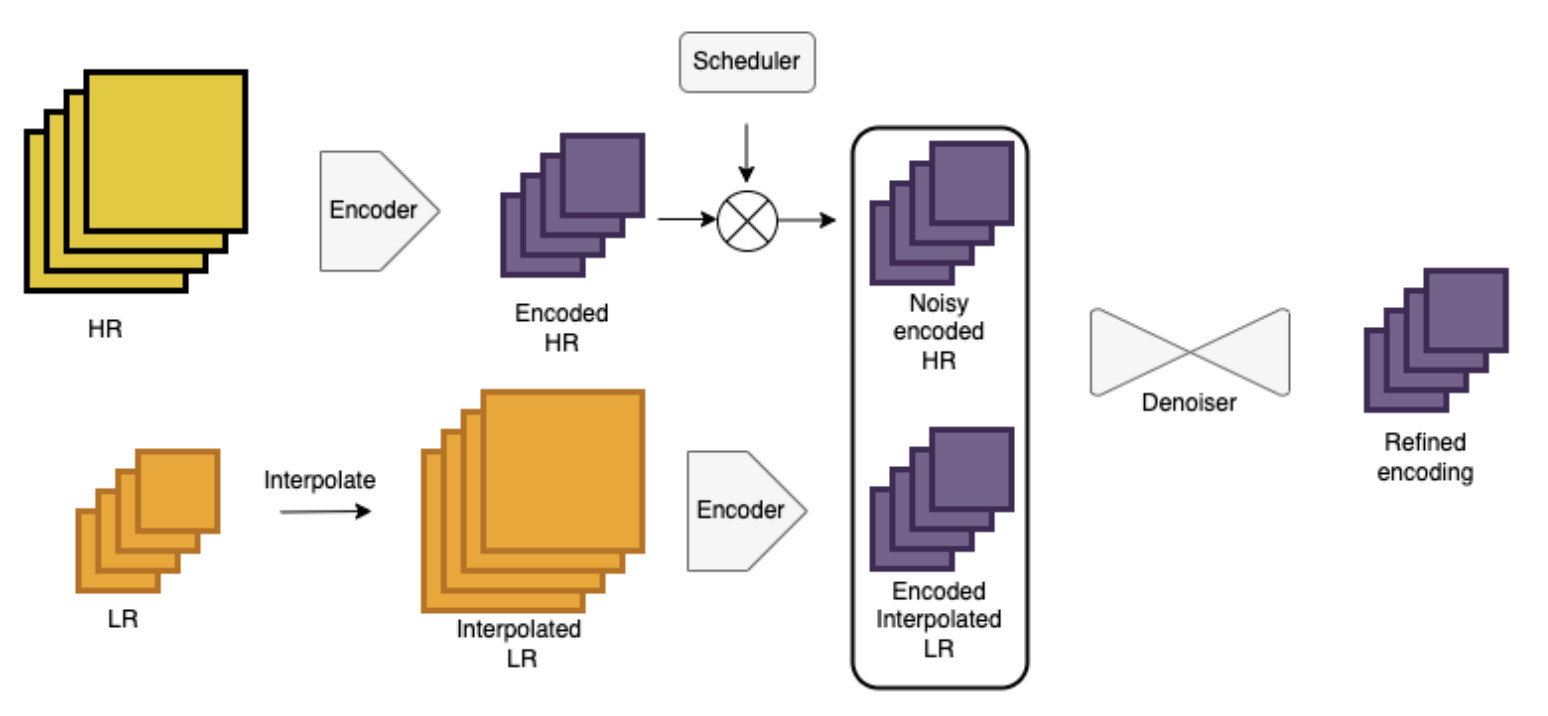
\includegraphics[width=1\linewidth]{images/simon/encLR_schema.png}
    \begin{justify}
        \textit{Nota.} Esquema de los cambios en el flujo de trabajo de SR del UNet. La eliminación de ruido se condiciona en una imagen $LR$ interpolada y codificada en lugar de en la imagen $LR$ original.
    \end{justify}                    
    \label{fig:encLR_schema}
\end{figure}

\begin{figure}[H]
    \caption{\doublespacing \\ \textit{Visualización de una versión interpolada (izquierda), codificada (centro) y decodificada (derecha) de la misma imagen.}} 
    \centering
    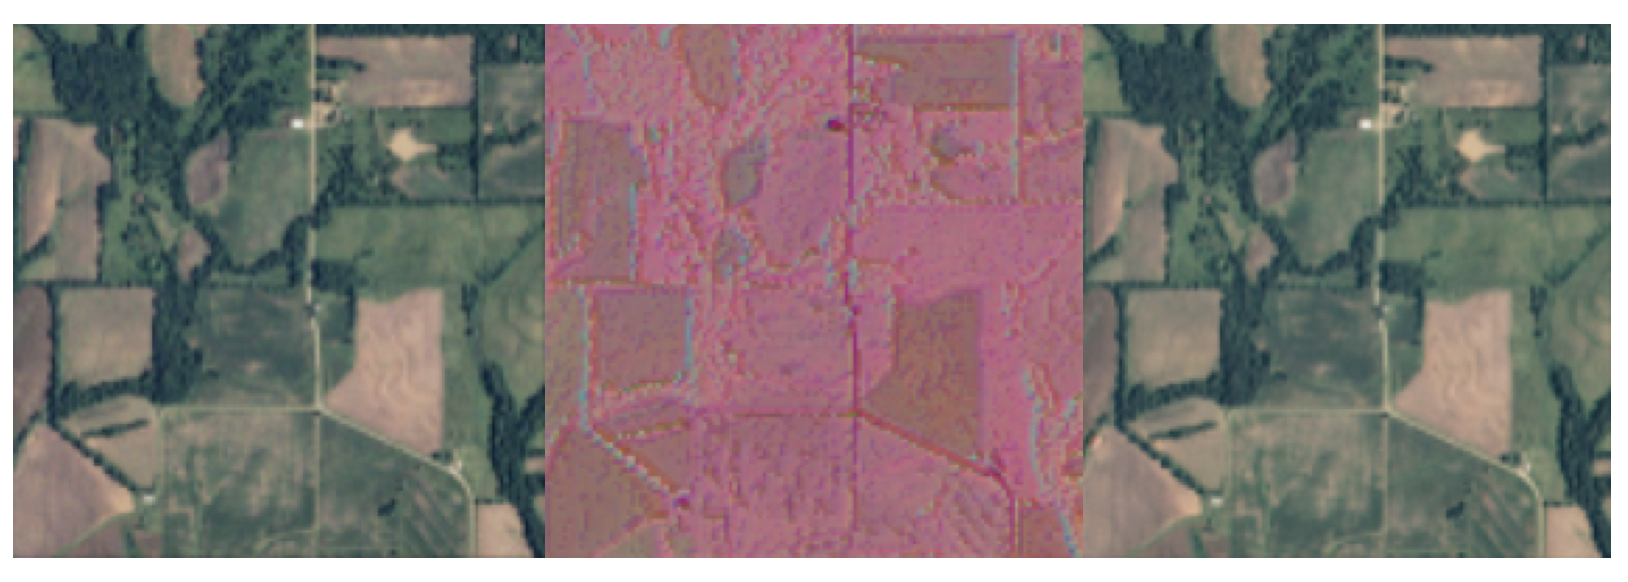
\includegraphics[width=1\linewidth]{images/simon/encLRint_demo.png}
    \begin{justify}
        \textit{Nota.} Visualización de una versión interpolada (izquierda), codificada (centro) y decodificada (derecha) de la misma imagen. Esto demuestra que el AE, aunque entrenado en imágenes $HR$, puede procesar con precisión imágenes $LR$ interpoladas.
    \end{justify}                    
    \label{fig:encLRint_demo}
\end{figure}

\subsection{Metodología SISR Multiespectral de Bandas de 20m}
Las metodologías previas describen el rendimiento de la SR de 4 bandas RGB-NIR en el conjunto de datos S2NAIP. Para realizar SR en las bandas de 20m de Sentinel-2, son necesarias ciertas adaptaciones. 

Si bien este conjunto de datos no coincide exactamente con las características espectrales de las bandas de 20m de Sentinel-2, ya está adaptado entre $LR$ y $HR$, está co-registrado espacialmente y degradado utilizando núcleos de degradación optimizados para esta tarea. Como el entrenamiento se realiza con permutaciones y orden aleatorio de las bandas, los modelos idealmente aprenden los núcleos de degradación y las frecuencias espaciales presentes en las bandas de 20m, sin importar las bandas específicas.

Se entrena un autoencoder de 6 bandas en el conjunto de datos descrito, seguido por el entrenamiento de un U-Net de 6 bandas para realizar la tarea de SR. Estos cambios requieren un entrenamiento desde cero. 


\begin{table}[H]
    \caption{\doublespacing \\ \textit{Tipos de modelos para las diferentes bandas MSI de Sentinel-2.}}
    \begin{spacing}{8}
        \fontsize{8pt}{2pt}\selectfont  
        \begin{tabularx}{\linewidth}{P{6cm}*{4}{c}} 
            \toprule
            \textbf{Número de Banda} & \textbf{Descripción de la Banda} & \textbf{Resolución (m)} & \textbf{Tipo de Modelo} \\
            \midrule
            B1 & Aerosol costero & 60 & - \\
            B2 & Azul & 10 & Modelo de 4 bandas \\
            B3 & Verde & 10 & Modelo de 4 bandas \\
            B4 & Rojo & 10 & Modelo de 4 bandas \\
            B5 & Borde rojo de vegetación & 20 & Modelo de 6 bandas \\
            B6 & Borde rojo de vegetación & 20 & Modelo de 6 bandas \\
            B7 & Borde rojo de vegetación & 20 & Modelo de 6 bandas \\
            B8 & Infrarrojo cercano (NIR) & 10 & Modelo de 4 bandas \\
            B8A & NIR estrecho & 20 & Modelo de 6 bandas \\
            B9 & Vapor de agua & 60 & - \\
            B10 & SWIR - Cirrus & 60 & - \\
            B11 & Infrarrojo de onda corta (SWIR) & 20 & Modelo de 6 bandas \\
            B12 & Infrarrojo de onda corta (SWIR) & 20 & Modelo de 6 bandas \\
            \bottomrule
        \end{tabularx}
    \end{spacing}
    \vspace{1\baselineskip}
    \textit{Nota.} Tipos de modelos utilizados para las diferentes bandas MSI de Sentinel-2.
    \label{table:sentinel2_bands_model}
\end{table}

\section{Estrategia de Entrenamiento SISR}
Los conjuntos de datos utilizados en este estudio y sus propiedades se detallan en \autoref{chapter:datasets}. Esta sección describe cómo se aprovechan estos conjuntos de datos durante el proceso de entrenamiento de los modelos de SR. Debido al alto número de parámetros del autoencoder y del U-Net de eliminación de ruido, se requieren grandes cantidades de datos de entrenamiento. Los autores originales \autocite{rombach2022highresolution} entrenaron sus modelos utilizando el conjunto de datos OpenImages, que contiene millones de imágenes. Para tareas de superresolución RGB, es posible ajustar los puntos de control optimizados de estos autores utilizando imágenes de teledetección. A pesar de la disponibilidad limitada de imágenes de entrenamiento en este dominio, el ajuste fino puede ser suficiente para esta tarea.

\paragraph{SISR RGB-NIR}
Para la superresolución RGB-NIR, se requiere entrenamiento desde cero, ya que no existen modelos preentrenados disponibles para entrada de 4 bandas. Por lo tanto, se necesitan grandes conjuntos de datos. La siguiente estrategia de entrenamiento utiliza diferentes conjuntos de datos de manera secuencial para aprovechar al máximo sus fortalezas:

\begin{enumerate}
    \item \textit{Conjunto de datos de imágenes naturales de CV}: Este conjunto de datos, compilado para este proyecto, contiene aproximadamente 280,000 imágenes. Aunque solo incluye imágenes RGB, generamos la cuarta banda faltante añadiendo el nivel de intensidad de la imagen como la cuarta banda. Este método no es idéntico a la banda NIR, pero proporciona información espacial y espectral útil, ya que el nivel de intensidad se normaliza al mismo rango que los otros conjuntos de datos.
    \item \textit{Conjunto de datos degradado de Sentinel-2}: Después del entrenamiento inicial con imágenes naturales, se utilizan datos de teledetección. Este conjunto de datos incluye 240,000 imágenes, aunque carece de las propiedades espaciales específicas para la pregunta de investigación, ya que la versión $LR$ tiene una resolución de 40m y la versión $HR$ de 10m. Sin embargo, al consistir en imágenes de teledetección con las mismas propiedades espectrales que los datos de Sentinel-2, ayuda a entrenar el modelo en características espectrales y espaciales relevantes.
    \item \textit{Conjunto de datos NAIP}: Este conjunto de datos se asemeja mucho tanto a las propiedades espaciales como espectrales de los datos de Sentinel-2. La versión $LR$ tiene una resolución de 2.5 metros, que coincide con las características espectrales del sensor Sentinel-2, mientras que la versión $HR$ es de 2.5 metros. Con 250,000 imágenes, este conjunto de datos es suficiente por sí solo para el entrenamiento desde cero. Sin embargo, el preentrenamiento en conjuntos de datos anteriores hace que los modelos sean más robustos.
    \item \textit{Conjunto de datos Worldstrat}: Con solo 3,000 imágenes, este conjunto de datos es demasiado pequeño para el entrenamiento independiente o el ajuste fino, ya que el modelo se sobreajustará. Además, utiliza un enfoque de sensor cruzado, lo que complica la verificación de los resultados sintéticos. Los modelos SISR finales no se entrenan en este conjunto de datos.
\end{enumerate}

\paragraph{SISR Multiespectral de Bandas de 20m}
El modelo de 6 bandas sigue una estrategia de entrenamiento similar. Al generar conjuntos de datos sintéticos de 6 bandas S2NAIP, el proceso de entrenamiento se mantiene consistente mediante estrategias de repetición y permutación. El entrenamiento procede de la siguiente manera:

\begin{enumerate}
    \item \textit{Conjunto de datos de imágenes naturales de CV}: Este conjunto de datos sirve como la fase inicial de entrenamiento, aprovechando su abundante cantidad de datos.
    \item \textit{Conjunto de datos degradado de Sentinel-2}: Después del preentrenamiento, el modelo se refina en datos de Sentinel-2 para centrarse en las características de imagen específicas del satélite. Sin embargo, la interpolación y SR de 80m a 20m introduce desafíos con diferentes núcleos de degradación.
    \item \textit{Conjunto de datos NAIP}: Las 250,000 imágenes de este conjunto de datos sirven como la mejor aproximación para el problema de degradación en cuestión, con similitudes espaciales y espectrales que lo hacen ideal para entrenar los modelos de SR.
\end{enumerate}

Estas estrategias de entrenamiento permiten que los modelos de 4 bandas y de 6 bandas evolucionen gradualmente, pasando de un enfoque general de reconstrucción de imágenes y SR hacia los requisitos espaciales y espectrales específicos de la pregunta de investigación.

\subsection{Datos de Sensor Cruzado vs Sintéticos}
Se han propuesto varias técnicas de aprendizaje profundo para superresolución en la observación de la Tierra \autocite{wang2022review, liu2021research, sdraka2022deep}. Estos métodos se clasifican en enfoques de sensor cruzado y enfoques sintéticos. Los algoritmos de sensor cruzado requieren un cuidadoso alineamiento espacial y coincidencia espectral de pares $HR$ y $LR$, a menudo restringidos por la necesidad de grandes conjuntos de datos. Los métodos sintéticos, por otro lado, generan imágenes $LR$ degradando imágenes $HR$ mediante un núcleo de desenfoque y submuestreo, aunque las brechas de dominio entre los datos sintéticos y los del mundo real siguen siendo un desafío \autocite{dong2022real, qiu2023cross, zhang2022single}.
